\documentclass[crop,tikz]{standalone}
\usetikzlibrary{backgrounds}
\colorlet{blue}{cyan}
\tikzset{
  inverted/.style = {
    color=white,
    background rectangle/.style={fill},
    show background rectangle
  }
}

\tikzset{>=latex}

\begin{document}
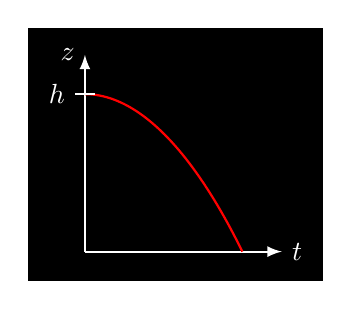
\begin{tikzpicture}[inverted,scale=2.5,thick]
  \draw[->] (0,0) -- (1,0) node[right] {$t$};
  \draw[->] (0,0) -- (0,1) node[left] {$z$};
  \draw[red] (0,0.8) parabola bend (0,0.8) (0.8,0);
  \draw (-0.05,0.8) node[left] {$h$} -- (0.05,0.8);
\end{tikzpicture}
\end{document}
